\documentclass[10pt, conference, a4paper, final]{IEEEtran}
\IEEEoverridecommandlockouts
\usepackage{amsmath, amssymb}
\usepackage[margin=1in]{geometry} % Adjust margins if needed
\usepackage{graphicx} % Required for including images
\usepackage{subcaption}
\usepackage{algorithm, algorithmicx} % For algorithms
\usepackage[table,xcdraw]{xcolor} % For colored tables
\usepackage{enumitem} % For better control over list
\usepackage{microtype} % Improves typography
\usepackage{amsmath}

% Combine graphicx package loading
\usepackage{float}
\usepackage{booktabs} % For professional looking tables

\title{Local and Global Coverage Assessment of Deep Learning Models}
\author{Author Name}
\date{\today}

\begin{document}

\maketitle

\begin{abstract}
% Your abstract goes here.
\end{abstract}


\section{Introduction}

\section{Problem Statement}
Deep learning models are increasingly integral to a vast range of applications, from automated driving systems to medical diagnostics. However, ensuring these models perform reliably under diverse and unexpected conditions remains a significant challenge. Current methods often lack the comprehensiveness and systematic approach needed to fully evaluate model robustness, particularly when facing real-world variations in data. This research addresses the critical gap by developing a robust methodology that not only evaluates model performance across standard metrics but also delves into the nuanced dynamics of error summarization. The goal is to establish a systematic framework that identifies and quantifies local and global robustness, providing a detailed error analysis that guides improvements in model design and training. This framework aims to elevate the trustworthiness and reliability of deep learning models, ensuring they meet the rigorous demands of practical applications.

\section{Contributions}
This research makes the following key contributions to the field of deep learning robustness evaluation:
\begin{itemize}
    \item Developed an \textbf{end-to-end pipeline} for systematically testing and evaluating the robustness of convolutional neural networks, focusing on the MNIST dataset.
    \item Introduced a novel methodology for \textbf{error summarization} that quantifies both local and global robustness, enhancing the identification of model vulnerabilities specific to class and property.
    \item Implemented advanced \textbf{sampling techniques} and \textbf{Bayesian updating methods} to refine the assessment of model robustness dynamically based on test outcomes.
    \item Formalized the impact of \textbf{class-specific behaviors} on model robustness through mathematical formalizations, providing a clear framework for identifying and addressing sources of error.
    \item Created a \textbf{comprehensive graphical representation} that visually summarizes the relationships and impacts between classes, properties, and their roles in model robustness.
\end{itemize}

\section{Research Questions}
This research seeks to address the following questions to enhance robustness evaluation frameworks applicable to various deep learning models and datasets:
\begin{itemize}
    \item How can we design a comprehensive and adaptable framework that integrates sampling, test case generation, and error analysis phases to ensure thorough robustness evaluation of deep learning models?
    \item How can robustness be systematically specified and evaluated at both local (property-specific) and global (overall model) levels within deep learning models?
    \item How can probabilistic graphical model be integrated into systematic testing frameworks to enhance the evaluation of local and global robustness in deep learning?
    \item  How can error summarization trace and quantify influences on a model’s overall robustness?
 
\end{itemize}



\section{Methodology}
\begin{figure*}{}
    \centering
    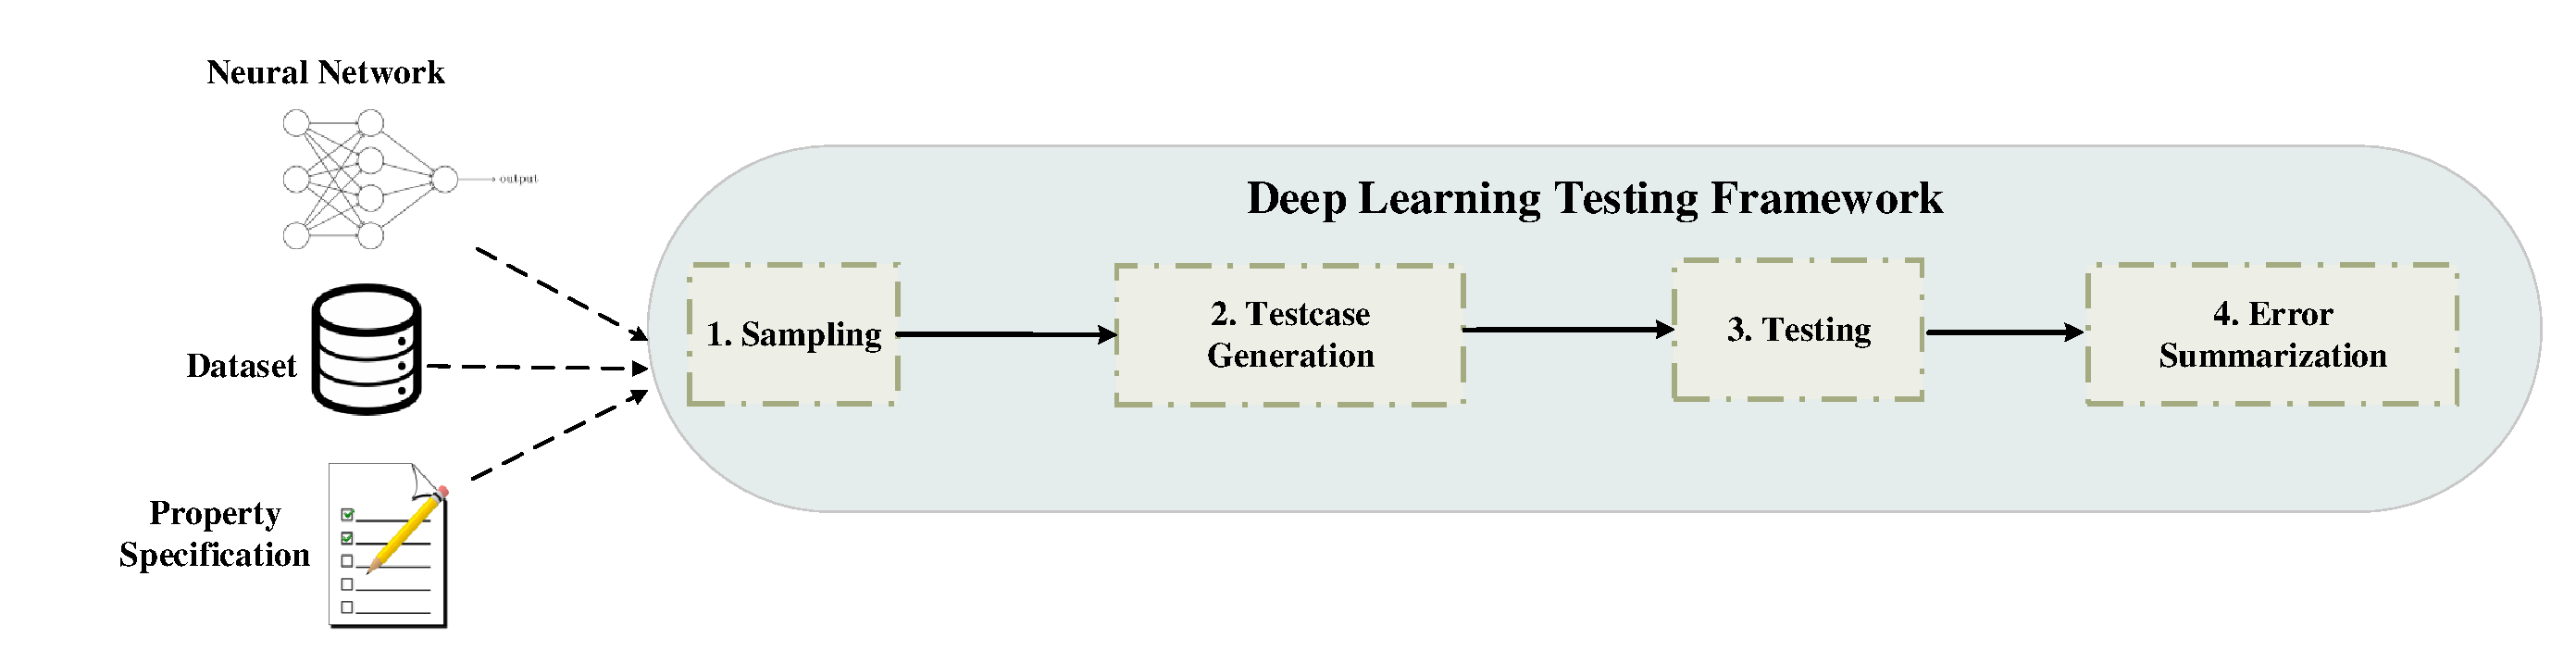
\includegraphics[width=\linewidth]{paper_images/DL framework.pdf}
    \caption{Graphical Representation}
    \label{fig:graph}
\end{figure*}

This section provides an overview of the comprehensive testing framework designed to verify and test the specified properties according to user requirements. The pipeline begins by clearly defining the properties that need to be assessed. Test cases are generated and tested/verified following the specification to evaluate the model rigorously. The error summarization phase then examines these results, focusing on the progression from local to global robustness to highlight the systemic strengths and vulnerabilities of the model. This systematic approach enhances the reliability and robustness of deep learning models by systematically addressing each critical aspect, from specification through comprehensive error analysis.

\subsubsection{Sampling}
This subsection details the sampling techniques employed using the MNIST dataset, a large database of handwritten digits commonly used in training and testing in the field of machine learning. Key steps in the sampling process include:

\begin{itemize}
    \item \textbf{Model Utilization:}
        \begin{itemize}
            \item A pre-trained Convolutional Neural Network (CNN) model, trained on the MNIST dataset, was utilized to select initial samples.
            \item Let \( X = \{x_1, x_2, \dots, x_N\} \) represent the entire MNIST dataset where each \( x_i \) is an image. The model's function \( f \) predicts the label \( y_i \) for each image \( x_i \):
            \[ f(x_i) \rightarrow y_i \]
            \item The model's outputs were analyzed to identify images that were predicted with complete accuracy, filtering to include only those examples that were correctly classified. This is defined by the filtering function \( g \), where:
            \[ g(x_i) = 
            \begin{cases} 
            1 & \text{if } f(x_i) = \text{true label of } x_i \\
            0 & \text{otherwise}
            \end{cases} \]
            \item The subset \( S \) of selected samples from \( X \) is thus:
            \[ S = \{x_i \in X \mid g(x_i) = 1\} \]
            This subset \( S \) contains images correctly identified by the model, ensuring the integrity and reliability of the samples for further testing.
        \end{itemize}
    \item \textbf{Random Selection of Samples:}
        \begin{itemize}
            \item To ensure a balanced representation, 200 samples from each digit class (0 through 9) were randomly selected from \( S \), resulting in a total of 2000 samples. This maintains an equal distribution across all classes.
            \item Let \( R \) represent the random selection function, ensuring that:
            \[ R(S, 200) = \text{randomly selects 200 samples from } S \]
            \[ \text{for each class} \]
        \end{itemize}
    \item \textbf{Criteria for Sample Selection:}
        \begin{itemize}
            \item The selection criteria are designed to achieve a statistically significant, evenly distributed set of data points.
            \item This approach supports a comprehensive evaluation of the model’s performance and robustness across varied input types.
        \end{itemize}
\end{itemize}

This methodological approach, formalized through the functions \( f \), \( g \), and \( R \), supports detailed examination and robustness testing by providing a controlled yet diverse set of inputs for subsequent phases of the pipeline.


\subsubsection{Test Case Generation}
This subsection describes the methodology for generating test cases designed to assess the robustness of a pre-trained Convolutional Neural Network (CNN) model on the MNIST dataset against various types of image distortions, including noise and geometric transformations. The generated test cases are specifically aligned with the properties that were specified earlier in the pipeline—noise resilience and geometric stability. Detailed steps include:

\begin{itemize}
    \item \textbf{Noise Addition:}
        \begin{itemize}
            \item \textit{Purpose:} To evaluate the model's performance when random visual noise is introduced, which mimics the effect of poor image quality typically found in real-world settings.
            \item \textit{Method:} Random Gaussian noise is added to the images from the selected subset \( S \). Define the noise function \( p_n(x_i, \sigma) \) where \( \sigma \) controls the intensity and variance of the noise:
            \[ x'_i = p_n(x_i, \sigma) \]
            where \( x'_i \) represents the image \( x_i \) after noise addition.
        \end{itemize}

    \item \textbf{Geometric Transformations:}
        \begin{itemize}
            \item \textit{Purpose:} To test the model's ability to accurately recognize digits under various geometric alterations, ensuring its effectiveness across different physical conditions and orientations.
            \item \textit{Method:}
                \begin{itemize}
                    \item \textbf{Rotation:} Images are rotated by predetermined angles to assess the model's ability to maintain recognition accuracy despite changes in orientation. Define the rotation function \( p_r(x'_i, \theta) \) where \( \theta \) is the angle of rotation:
                    \[ x''_i = p_r(x'_i, \theta) \]
                    % \item \textbf{Scaling and Translation:} Images are scaled and translated using affine transformation techniques. Define the transformation function \( p_t(x''_i, s, t) \) where \( s \) is the scale factor and \( t \) represents translation parameters:
                    % \[ x'''_i = p_t(x''_i, s, t) \]
                    \item \textbf{Brightness Adjustment:} The brightness of images is altered by modifying the pixel intensity values. Define the brightness function \( p_b(x'''_i, b) \) where \( b \) controls the brightness level:
                    \[ x''''_i = p_b(x'''_i, b) \]
                \end{itemize}
        \end{itemize}
\end{itemize}

Each type of test case is meticulously crafted to ensure that it targets and challenges a specific aspect of the model’s robustness, as defined in the property specification phase. This systematic approach ensures comprehensive testing of the model’s capabilities, providing a robust measure of its performance across varied and challenging conditions.
\begin{figure}{}
    \centering
    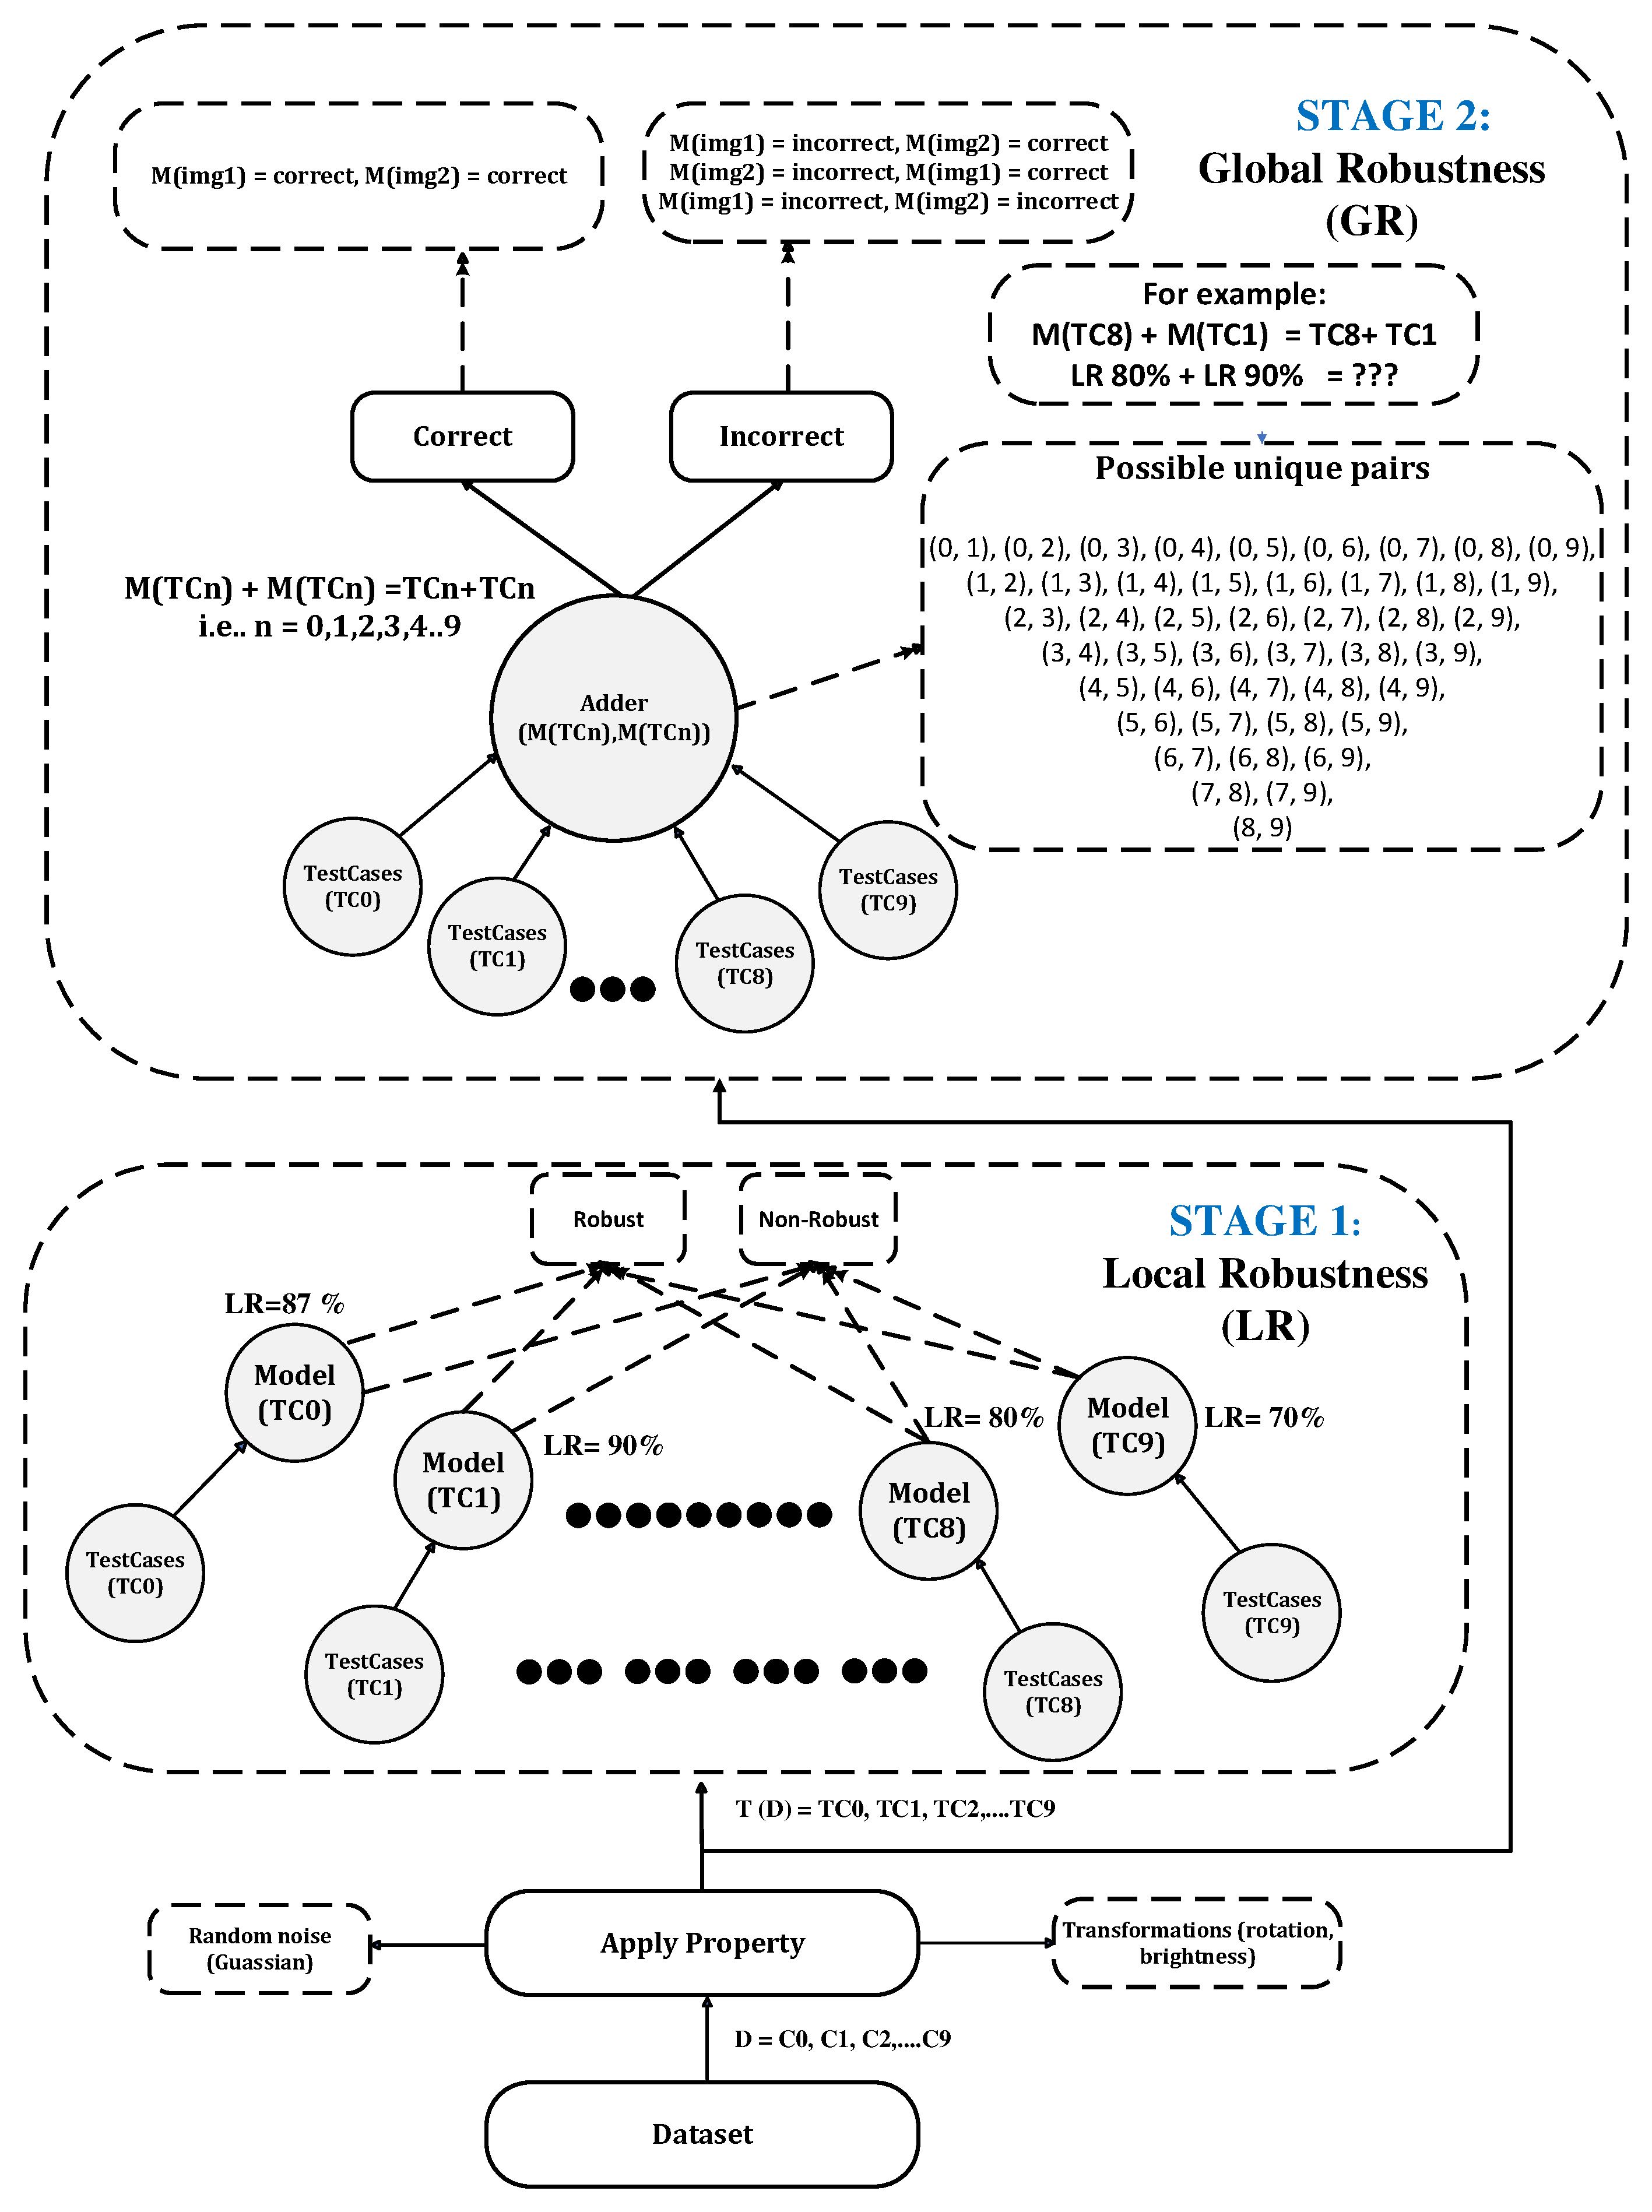
\includegraphics[width=\linewidth]{paper_images/MNIST Adder.pdf}
    \caption{Graphical Representation}
    \label{fig:graph}
\end{figure}
\subsubsection{Testing/Sampling}
This subsection outlines the procedures employed to assess the robustness of the pre-trained Convolutional Neural Network (CNN) model using the MNIST dataset against various image distortions, integrating Bayesian updating to enhance the precision of our robustness measurements.

\begin{itemize}
    \item \textbf{Local Robustness Testing (LR):}
        \begin{itemize}
            \item For each class \( c \) and each test case \( t \), model robustness is initially considered as a random variable with a prior distribution \( \pi(\theta_c) \), reflecting our belief in the model's robustness before observing test outcomes.
            \item As the model is subjected to distortions (noise, rotation, brightness adjustments), we collect data on the model's performance:
            \[ \text{Data}_c(t) = \{ \text{outcome of test } t \text{ on class } c\} \]
            \item Bayesian theoram is applied to adjust our belief based on the evidence from the test outcomes, recalculating the posterior probability of robustness:
            {\footnotesize\[
                \text{Posterior Robustness}_{\text{local}}(\theta_c | \text{Data}_c) =
                \frac{P(\text{Data}_c | \theta_c) \cdot \pi(\theta_c)}{P(\text{Data}_c)}
            \]}
      


            \item The posterior distribution informs us about the updated belief in the model’s robustness given the new data, thereby refining our understanding after each test case.
        \end{itemize}

        
    \item \textbf{Global Robustness Testing (GR):}
    \begin{itemize}
        \item Global robustness examines the model's performance when pairs of classes are tested together, simulating more complex, real-world scenarios:
        \[ \text{Adder}(x_{c1}, x_{c2}) = M(x_{c1}) + M(x_{c2}) \]
        
        \item For pairs of classes \( c1 \) and \( c2 \), we estimate the joint posterior probability that the model correctly recognizes both classes:
        {\footnotesize
        \begin{multline}
            \text{Robustness}_{\text{global}}(c1, c2) = \\
            \int \text{PR}_{\text{local}}(\theta_{c1}) \times \text{PR}_{\text{local}}(\theta_{c2}) \, d\theta_{c1} \, d\theta_{c2}
        \end{multline}
        }
        
        \item This integration over the posterior distributions from local robustness tests provides a probabilistic assessment of the model's capability to handle concurrent inputs, capturing the compounded uncertainties and dependencies between class recognitions.
    \end{itemize}
    
\end{itemize}

This approach, by continuously updating our beliefs about the model’s robustness through Bayesian inference, allows for a more dynamic and responsive evaluation process, ensuring each new piece of data refines our predictions and assessments.


\subsubsection{Error Summarization}
This subsection delves into the systematic analysis of errors identified during the testing phases, focusing on evaluating the model's robustness from a local and global perspective. The error summarization aims to pinpoint specific vulnerabilities related to individual classes and properties, thereby guiding targeted improvements in the model's architecture and training processes.

\paragraph{Mathematical Formalization}
Let us define the overall robustness, \( R_{\text{global}} \), as the weighted average of the local robustness scores of all properties, adjusted by their respective importance, \( w_i \):

\begin{equation}
    R_{\text{global}} = \sum_{i=1}^N w_i r_i
\end{equation}

where \( N \) is the total number of properties, \( r_i \) represents the robustness score of property \( i \), and \( w_i \) is the weight assigned to property \( i \), reflecting its significance in the overall system.

\paragraph{Local Robustness by Property and Class}
For each property \( i \) and class \( j \), let \( c_{ij} \) represent the confidence level of class \( j \) affecting property \( i \). The local robustness for each property is then computed as:

\begin{equation}
    r_i = \frac{1}{M_i} \sum_{j=1}^{M_i} c_{ij}
\end{equation}

where \( M_i \) is the number of classes that significantly impact property \( i \). This metric assesses how resilient each property is to variations in class-specific behavior.

\paragraph{Impact of Specific Classes}
We define a measure, \( \delta_{ijk} \), to capture the misclassification rate of class \( j \) for property \( i \) against a potentially confounding class \( k \):

\begin{equation}
    {\footnotesize
    \delta_{ijk} = \frac{\text{No. of misclassifications of class } j \text{ as class } k \text{ on property } i}{\text{Total no. of classifications of class } j \text{ on property } i}
    }
\end{equation}

This metric helps identify specific weaknesses in the model’s performance, particularly where certain classes are prone to misidentification under specific conditions.

\paragraph{Comprehensive Diagram}
To visually represent these concepts, a comprehensive diagram (see Figure \ref{fig:error-summarization}) can be employed, illustrating the relationships between different properties, classes, and their impact on local and global robustness. Nodes in the diagram represent classes and properties, while edges denote the significant impact of a class on a property, labeled by \( \delta_{ijk} \).

\begin{figure}[H]
    \centering
    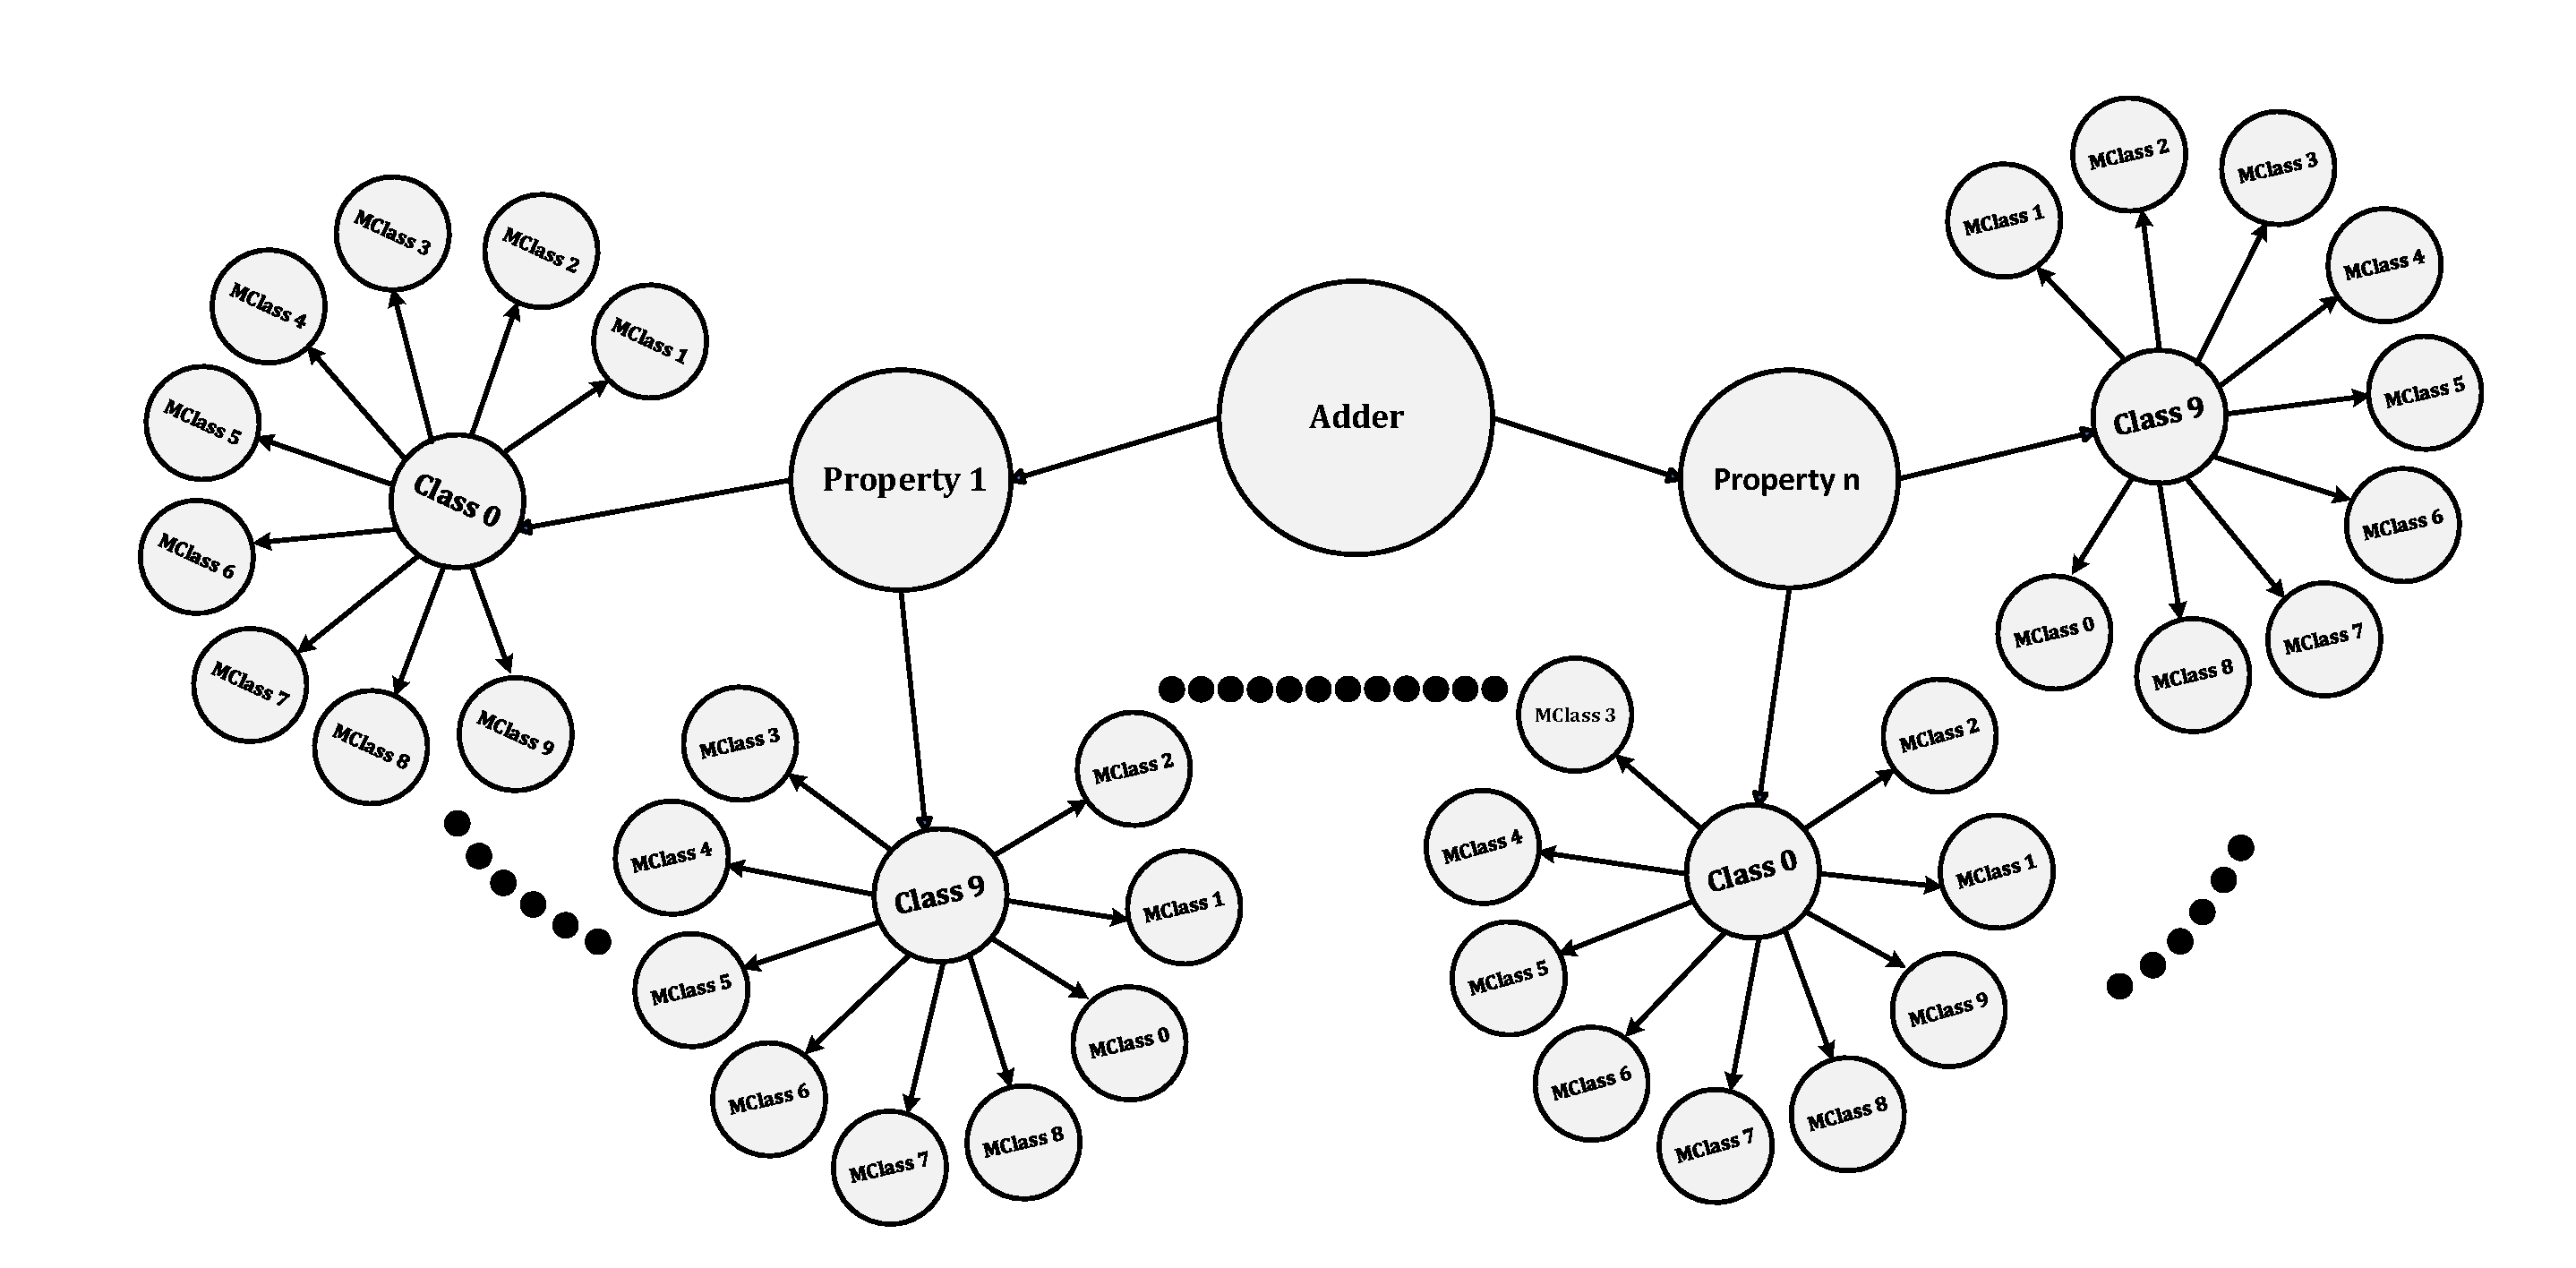
\includegraphics[width=\linewidth]{paper_images/step4.pdf}
    \caption{Diagram of Error Summarization Highlighting Class-Property Impact}
    \label{fig:error-summarization}
\end{figure}

This formalization not only aids in identifying the direct contributors to error but also assists in prioritizing areas for improvement based on their impact on the overall robustness of the system.


\section{Experiments}
% Your content here
\begin{itemize}
    \item How can we design a comprehensive and adaptable framework that integrates sampling, test case generation, and error analysis phases to ensure thorough robustness evaluation of deep learning models?
    \item How can robustness be systematically specified and evaluated at both local (property-specific) and global (overall model) levels within deep learning models?
    \item How can probabilistic graphical model be integrated into systematic testing frameworks to enhance the evaluation of local and global robustness in deep learning?
    \item  How can error summarization trace and quantify influences on a model’s overall robustness?
 
\end{itemize}

\section{Threats to Validity}

This section outlines significant limitations and assumptions in our study that may affect the validity and reliability of our findings.

\begin{itemize}
    \item \textbf{Random Sampling:} Our current approach assumes a uniform distribution of samples across all classes, which may not represent the true complexity and variability within real-world data. This uniform sampling can lead to biased evaluations if the class distribution in practical applications is skewed or non-uniform. We plan to enhance our sampling techniques to better capture the diversity and distribution of data in realistic scenarios. Improved sampling strategies will help in developing more robust and generalizable error summarization methods.
\end{itemize}


\section{Related Work}
% Your content here

\section{Conclusion}
% Your conclusion here

\begin{thebibliography}{01}
    \bibitem{Saad} Reference details
\end{thebibliography}

\end{document}
